\chapter{Descrizione del lavoro}
\label{descrizioeDelLavoro}
Per comprendere la soluzione proposta e il sistema ideato si utilizzerà un approccio top-down. Partendo da un livello d'astrazione tale in cui emergono solo i requisiti funzionali e il sistema è rappresentato da una \textit{black box}, si raggiunge un livello che permetterà di affinare i requisiti iniziali e mostrare i \textit{sottosistemi} che lo costituiscono. Infine nell'ultimo livello si avrà una visione dei \textit{moduli} che compongono i sottosistemi e che sono stati realizzati nel contesto di questa tesi.
\begin{figure}[H]
	\centering
	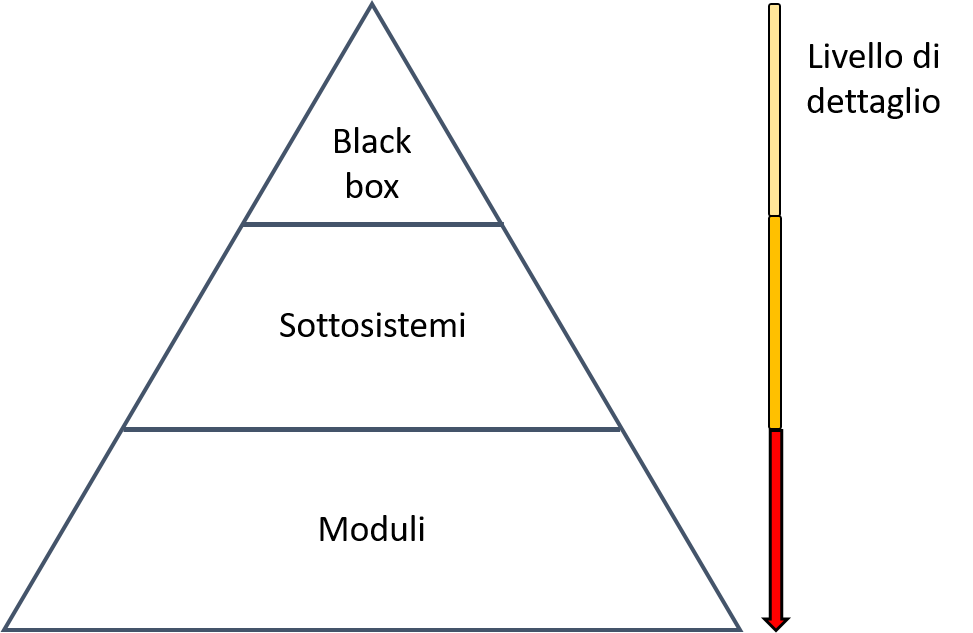
\includegraphics[scale=0.4]{DescrizioneDelSistema/livelli_astrazione.png}
	\caption{Rappresentazione dei livelli d'astrazione utilizzati per descrivere il sistema }
	\label{fig:livelliAstrazione}
\end{figure}
\newpage

\section{Livello black box}
Considerando il sistema in questione come una black box (Fig.\ref{fig:requisitiFunzionali}) e l'infrastruttura di rete in modo astratto, i due macro-requisiti funzionali  sono rispettivamente:
\begin{itemize}
	\item \textbf{R1}: Geolocalizzare l'operatore
	\item \textbf{R2}: Trasmettere messaggi predefiniti come stato della vittima e codici d'emergenza.
\end{itemize}
\begin{figure}[H]
	\centering
	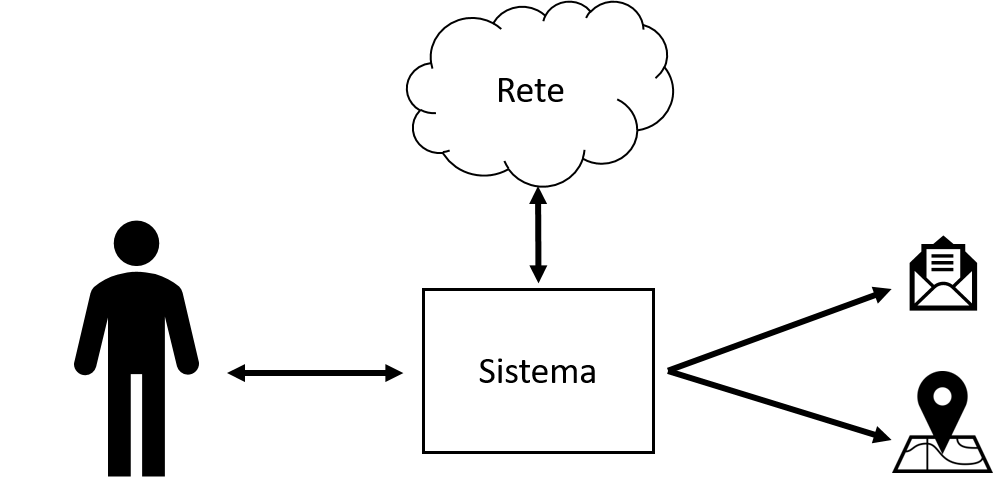
\includegraphics[scale=0.3]{DescrizioneDelSistema/requisitiSistema.png}
	\caption{Rappresentazione del sistema come black box }
	\label{fig:requisitiFunzionali}
\end{figure}
Nelle fasi primordiali del progetto, si è scelto di allocare la maggior parte delle risorse lavorative nel completamento di \textbf{R1} lasciando ad una fase successiva lo sviluppo di \textbf{R2}. \textit{R1} può essere suddiviso in due requisiti più specifici:
\begin{itemize}
	\item \textbf{R1.1}: Determinare la posizione di un operatore all'interno della rete
	\item \textbf{R1.2}: Identificare il cammino minimo da un operatore ad un altro
\end{itemize}
Quest'ultimo rappresenta sia la possibilità da parte dell'operatore di eseguire il percorso all'inverso, sia la possibilità che venga raggiunto da una squadra di supporto. A questo punto si può scendere al livello d'astrazione successivo (\ref{fig:livelliAstrazione}).
\newpage 


\section{Livello sottosistemi}
\label{livello_sottosistemi}
Per soddisfare il requisito \textbf{R1.1} è necessario che l'operatore si trovi all'interno di una zona \textit{infrastrutturata}, ovvero una zona dove i nodi della rete siano georeferenziati rispetto ad un sistema di riferimento comune. Considerata la modalità con la quale la rete è costruita, ovvero dinamicamente da un'esploratore,  garantire tale situazione non è un compito banale.\\
La soluzione si costruisce per iterazione georeferenziando i singoli nodi nel momento in cui vengono aggiunti dall'esploratore.\\
Con riferimento all'esempio illustrato precedentemente (Fig.\ref{fig:step1}- Fig.\ref{fig:step6}), si consideri lo step 2.
Per ipotesi si supponga che il primo nodo sia già georeferenziato, nel momento in cui l'operatore risulti essere al limite della line-of-sight e/o della distanza di sicurezza piazzerà il secondo nodo. \\
Per mantenere il livello d'astrazione attuale basta sapere che le caratteristiche della tecnologia utilizzata nell'implementazione della rete, fa si che le singole celle abbiano un raggio d'azione all'interno del quale il sottosistema \textit{S1} (Fig.\ref{fig:sistema_liv1}) può calcolare la distanza tra l'operatore e il centro della cella di appartenenza.\\
Tale informazione non è però sufficiente, infatti ci sono infiniti punti sulla circonferenza con centro nel primo nodo e raggio pari alla distanza. Per poter georeferenziare in modo univoco il secondo nodo si deve trovare anche l'angolo in riferimento al primo nodo.\\
La figura \ref{fig:ambiguitDistanz} rappresenta un tentativo di georeferenziare il secondo nodo utilizzando soltanto la distanza tra i due nodi.
\begin{figure}[H]
	\centering
	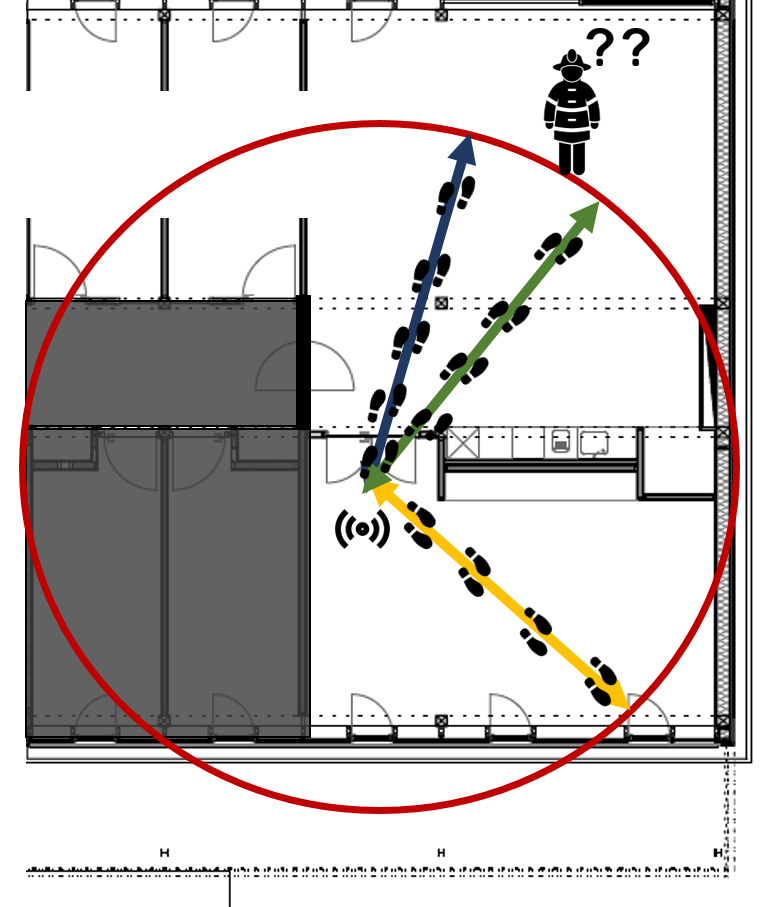
\includegraphics[scale=0.35]{DescrizioneDelSistema/ambiguitDistanza.png}
	\caption{Ambiguità nella georeferenziazione di un secondo nodo utilizzando soltanto la distanza dal precedente }
	\label{fig:ambiguitDistanz}
\end{figure}
Nell'esempio appena proposto, si sono mostrate solo tre delle possibili infinite posizioni del secondo nodo. Si assuma che il punto corretto sia l'intersezione tra il vettore in blu e la circonferenza. In tal caso un'ambiguità con il vettore in verde potrebbe essere accettata in quanto si discosta di pochi metri dalla reale posizione, ben diversa sarebbe un'ambiguità con il vettore in giallo che renderebbe l'informazione del tutto errata e il sistema disinformante.\\
In conclusione per georeferenziare in maniera univoca il nuovo nodo (rispetto al primo) sono necessarie le seguenti informazioni:
\begin{itemize}
	\item La distanza tra i due nodi
	\item L'angolo tra i due nodi
\end{itemize} 
Per ricavare queste informazioni si sono ideati due sottosistemi, rappresentati dalla Fig.\ref{fig:sistema_liv1}:
\begin{figure}[H]
	\centering
	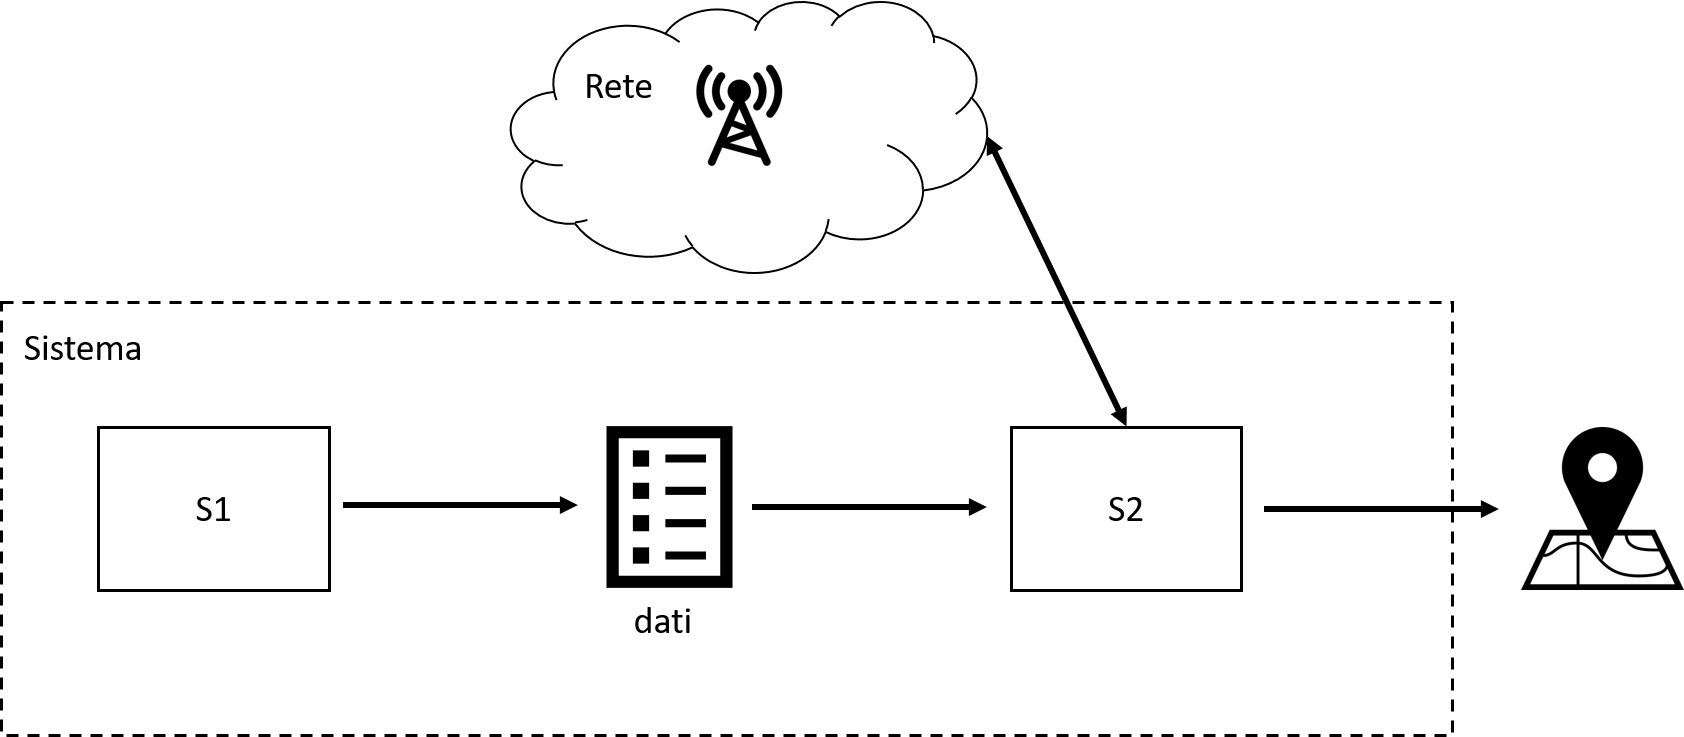
\includegraphics[scale=0.3]{DescrizioneDelSistema/sistema_liv1.png}
	\caption{Rappresentazione dei sottosistemi necessari per georeferenziare i nodi della rete }
	\label{fig:sistema_liv1}
\end{figure}
Ognuno dei quali con la propria responsabilità:
\begin{itemize}
	\item \textbf{S1}: ha il compito di ricavare tramite i sensori (cap.\ref{tecnologie}) le informazioni riguardanti gli angoli assunti dall'esploratore lungo il tragitto
	\item \textbf{S2}: ha il compito di ricevere i dati da S1 e la distanza dal nodo precedente, elaborarli e infine determinare la posizione del nuovo nodo
\end{itemize}

Relativamente alla rappresentazione del sistema mostrata in Fig.\ref{fig:sistema_liv1}, il lavoro di questi tesi si colloca nella progettazione e nello sviluppo del sottosistema S1.\\
Nel prossimo paragrafo si raggiungerà il livello d'astrazione più basso della piramide (vedi \ref{fig:livelliAstrazione}) dettagliando i moduli che compongono il sottosistema realizzato.\newpage


\section{Livello moduli}
\label{livello_moduli}
Prima di "aprire" il sottosistema è bene specificare che si utilizzerà il termine \textit{modulo} per riferirsi sia a componenti hardware che software. Questo abuso di notazione permetterà di mostrare con un unico livello d'astrazione tutti i moduli progettati e realizzati al fine di stimare gli angoli assunti dall'esploratore lungo il tragitto (si veda \ref{livello_sottosistemi}).
\begin{figure}[H]  
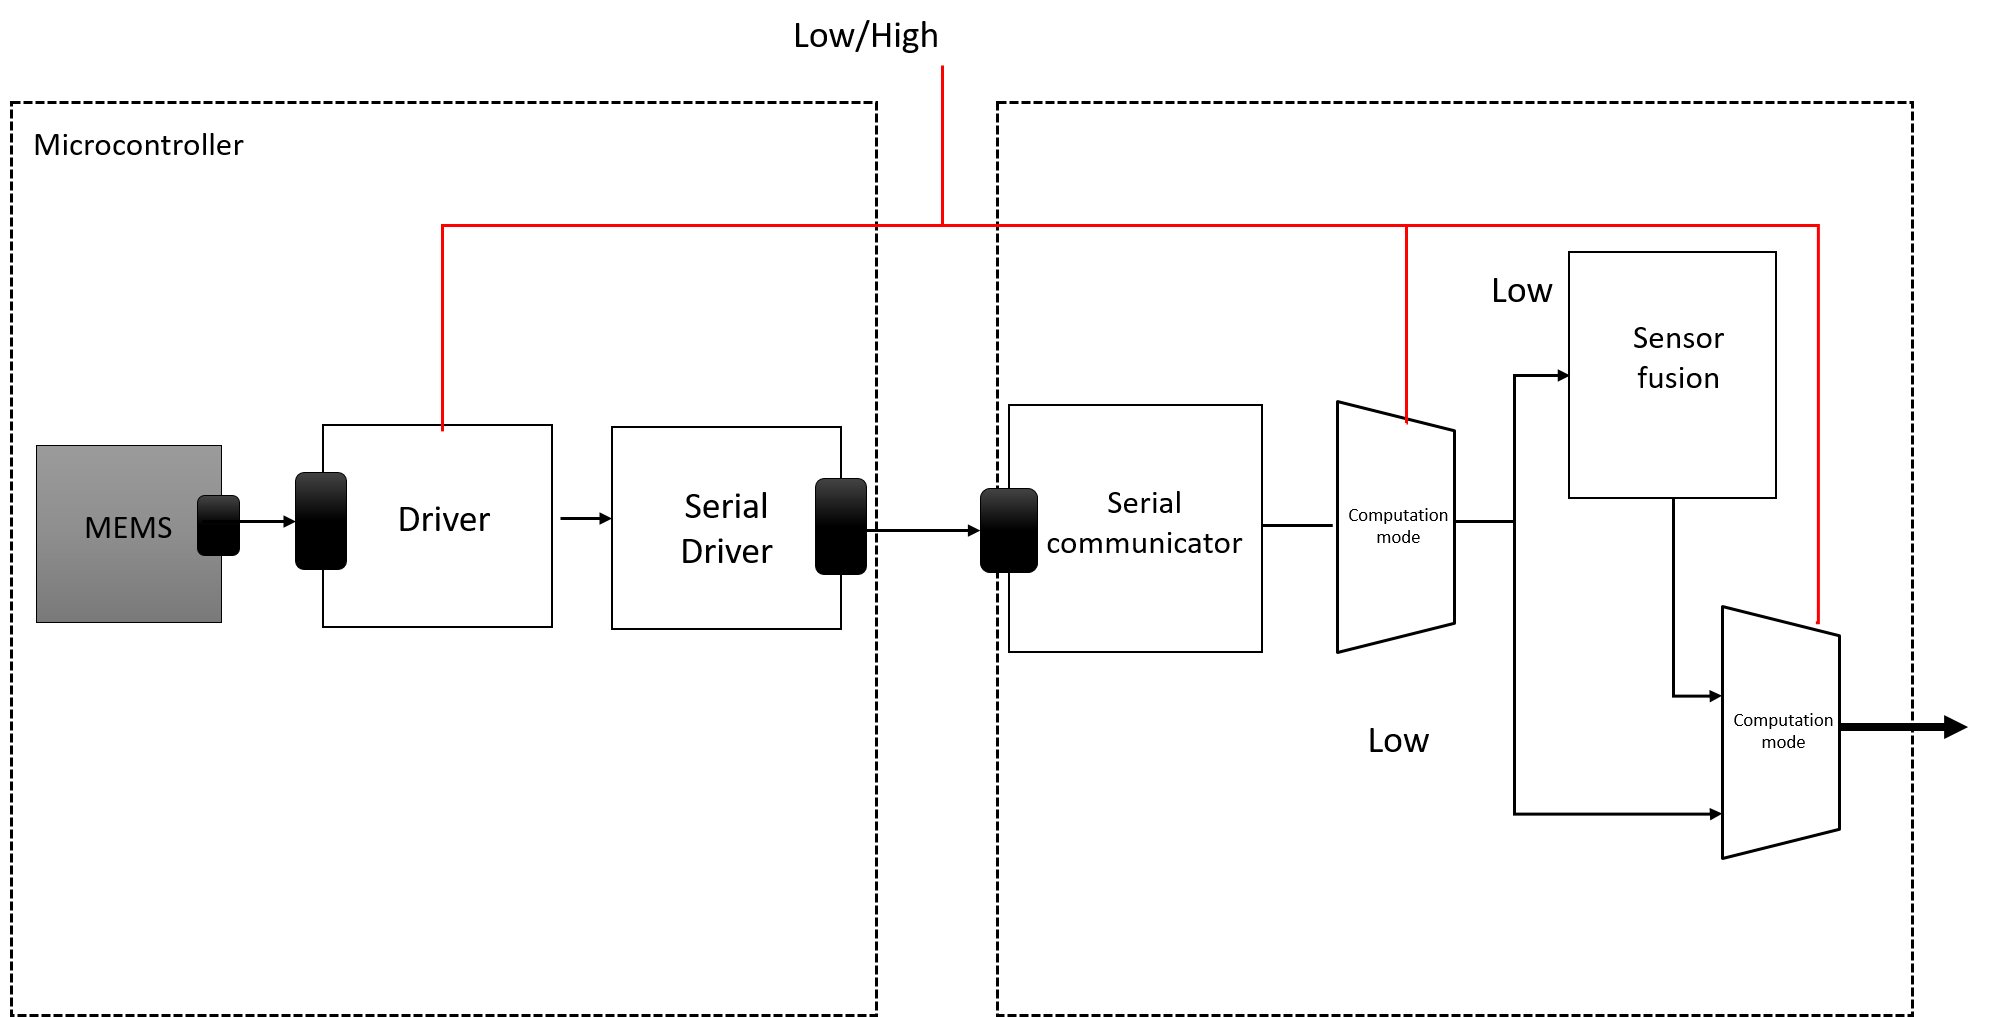
\includegraphics[scale=0.3 ]{DescrizioneDelSistema/sistema_liv2.png}
\caption{Rappresentazione dei sottosistemi in moduli}
\label{fig:sistema_liv2}
\end{figure}
Per esplicare al meglio i compiti dei singoli moduli e mantenere l'attuale livello d'astrazione, fermo restando che tutti i dettagli tecnici verranno forniti nei capitoli successivi, si mostrerà il flusso di dati generato in uno qualsiasi degli intervalli di campionamento lungo il tragitto dell'operatore tra un nodo e l'altro.\\ 
Il flusso inizia nel momento in cui il modulo \textit{driver} acquisisce le informazioni dall'unità \textit{MEMS} (cap.\ref{tecnologie}) riguardanti la velocità angolare, l'accelerazione e il campo magnetico relativi all'operatore. Come mostrato in Fig.\ref{fig:flusso1}. 
\begin{figure}[H] 
	\centering 
	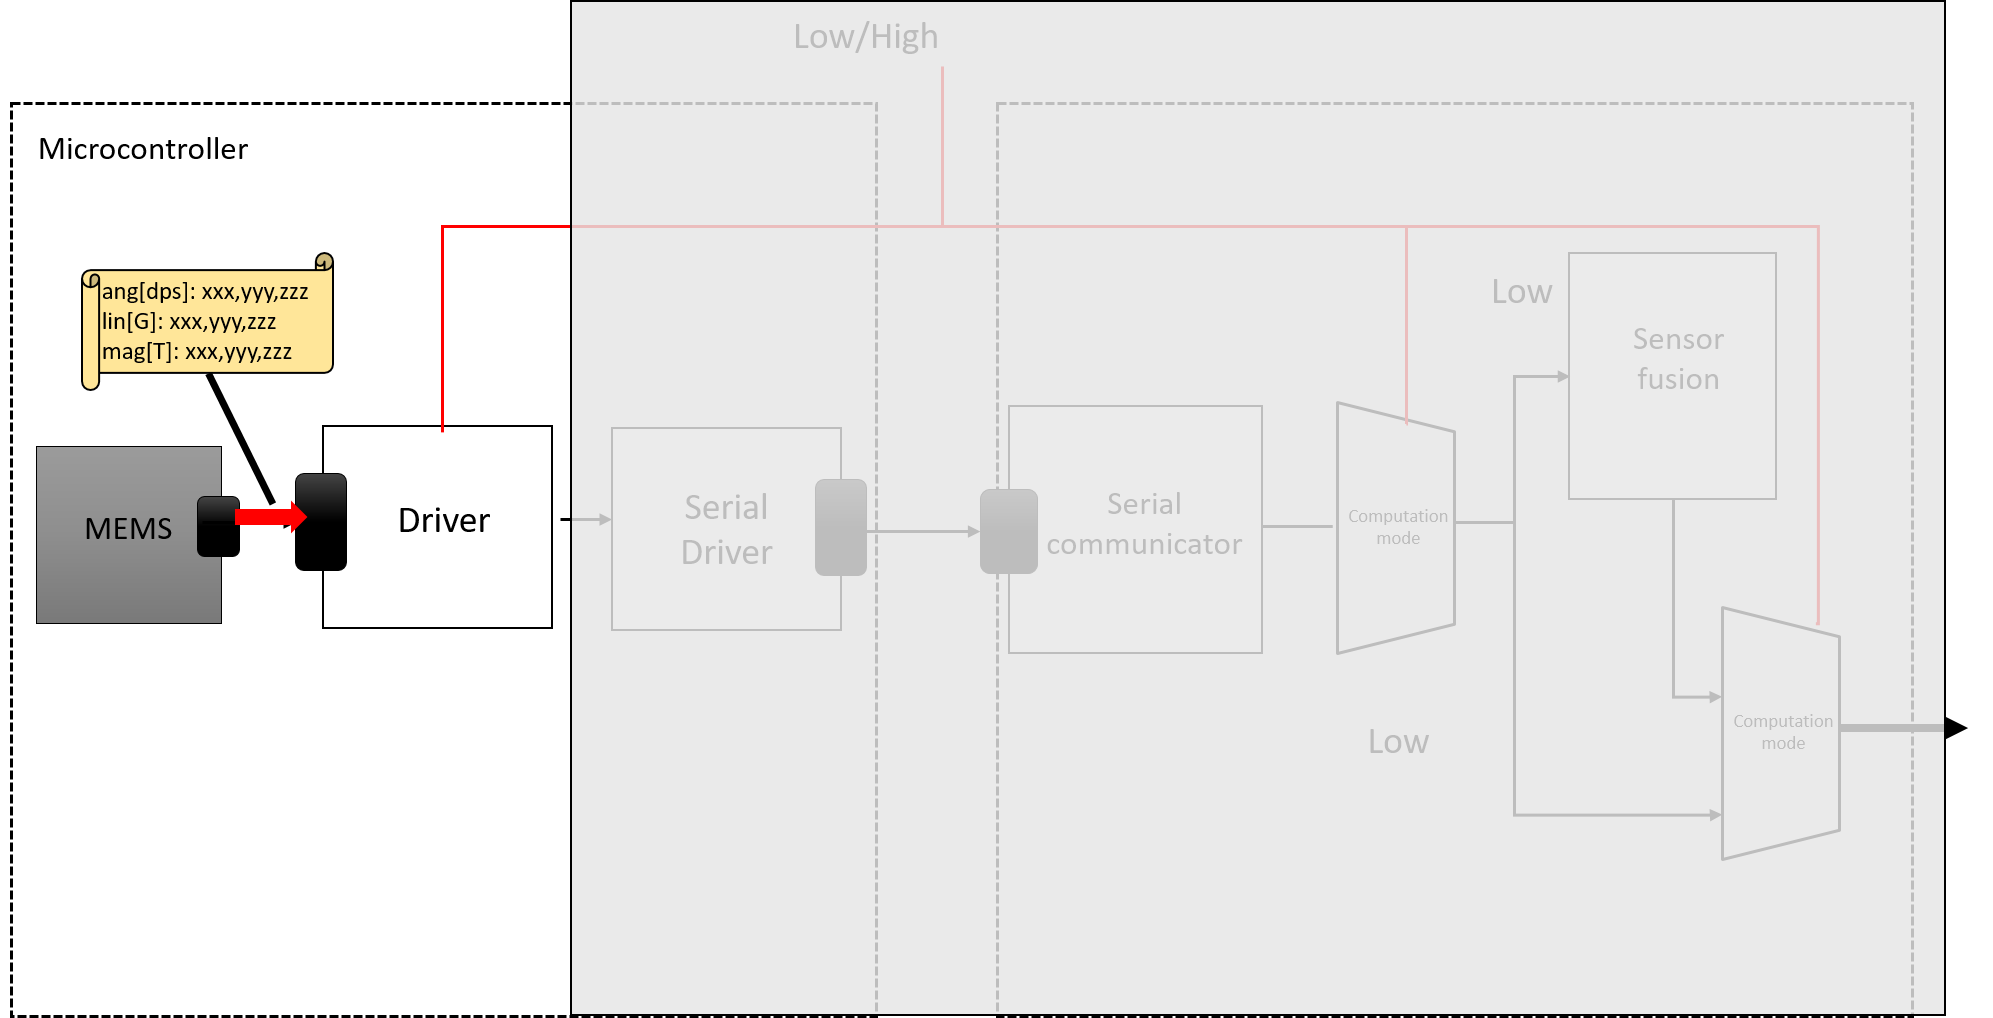
\includegraphics[scale=0.25 ]{DescrizioneDelSistema/flusso1.png}
	\caption{Rappresentazione del flusso di dati tra i moduli dei sottosistemi, step 1}
	\label{fig:flusso1}
\end{figure}
I dati acquisiti sono "grezzi" e devono essere elaborati (Cap.\ref{elaborazione}). Quando e da chi questa computazione verrà eseguita durante il flusso, viene stabilito attraverso il comando Low/High. Da questo ne consegue anche la modalità di funzionamento del driver in:
\begin{itemize}
	\item \textbf{HCM}: High Computation mode, i dati vengono elaborati dal microcontrollore
	\item \textbf{LCM}: Low Computation mode, i dati verranno elaborati in seguito dal sottosistema \textit{App} 
\end{itemize}
La scelta tra quale di queste due modalità utilizzare verrà motivata nel capitolo riguardante l'analisi dei risultati (cap.\ref{elaborazione}), per il momento si ipotizzi di settare la linea di comando al valore "Low" e quindi di utilizzare il driver in \textit{LCM}. Con queste impostazioni i dati grezzi vengono impacchettati ed etichettati con un timestamp relativo, prima di essere inviati dal modulo \textit{Serial driver} e ricevuti dal modulo \textit{App} mediante il modulo \textit{Serial communicator}, quest'ultimo li inoltra all'ingresso del multiplexer \textit{Computation mode} come mostrato in Fig.\ref{fig:flusso2}:
\begin{figure}[H]  
	\centering 
	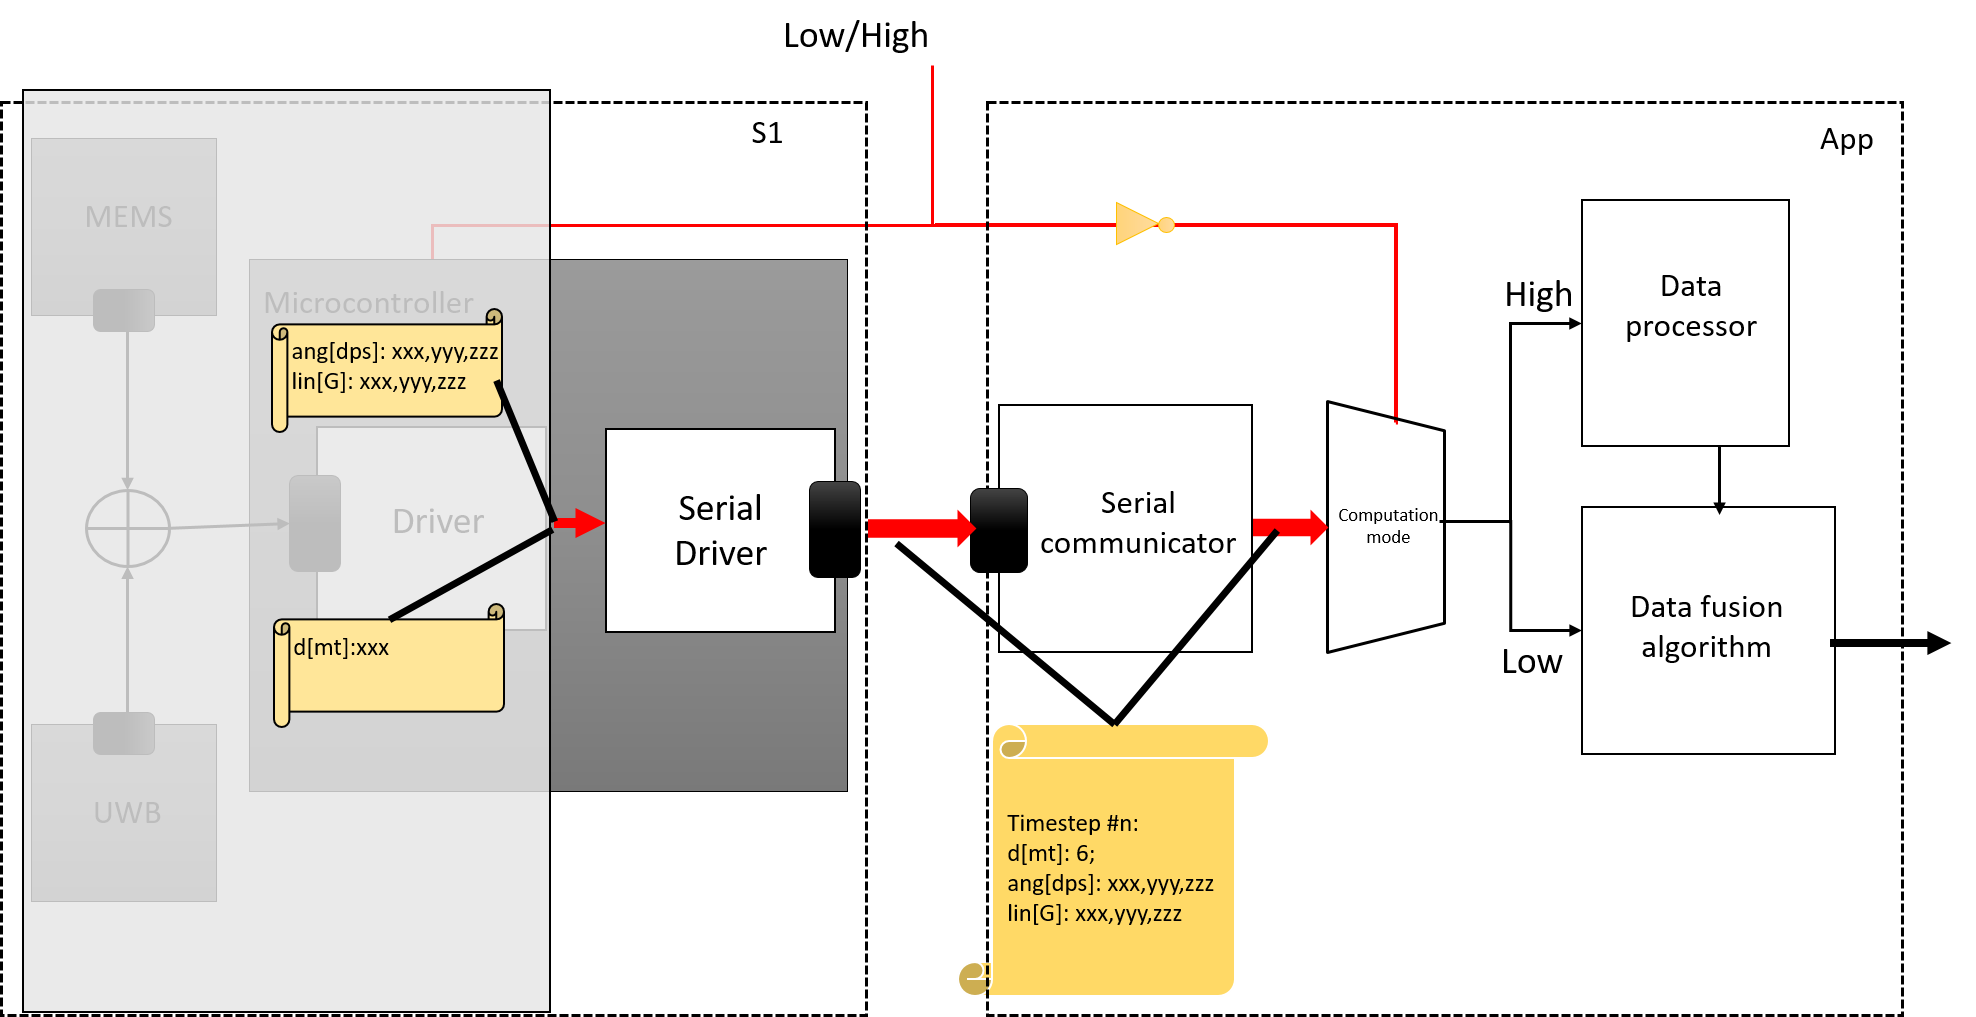
\includegraphics[scale=0.25 ]{DescrizioneDelSistema/flusso2.png}
	\caption{Rappresentazione del flusso di dati tra i moduli dei sottosistemi, step 2}
	\label{fig:flusso2}
\end{figure}
Poiché per ipotesi si è scelto di settare la linea di comando sul valore \textbf{Low}, il multiplexer devia il flusso di dati verso il modulo \textit{Sensor Fusion} come mostrato in figura:
 \begin{figure}[H]  
 	\centering 
 	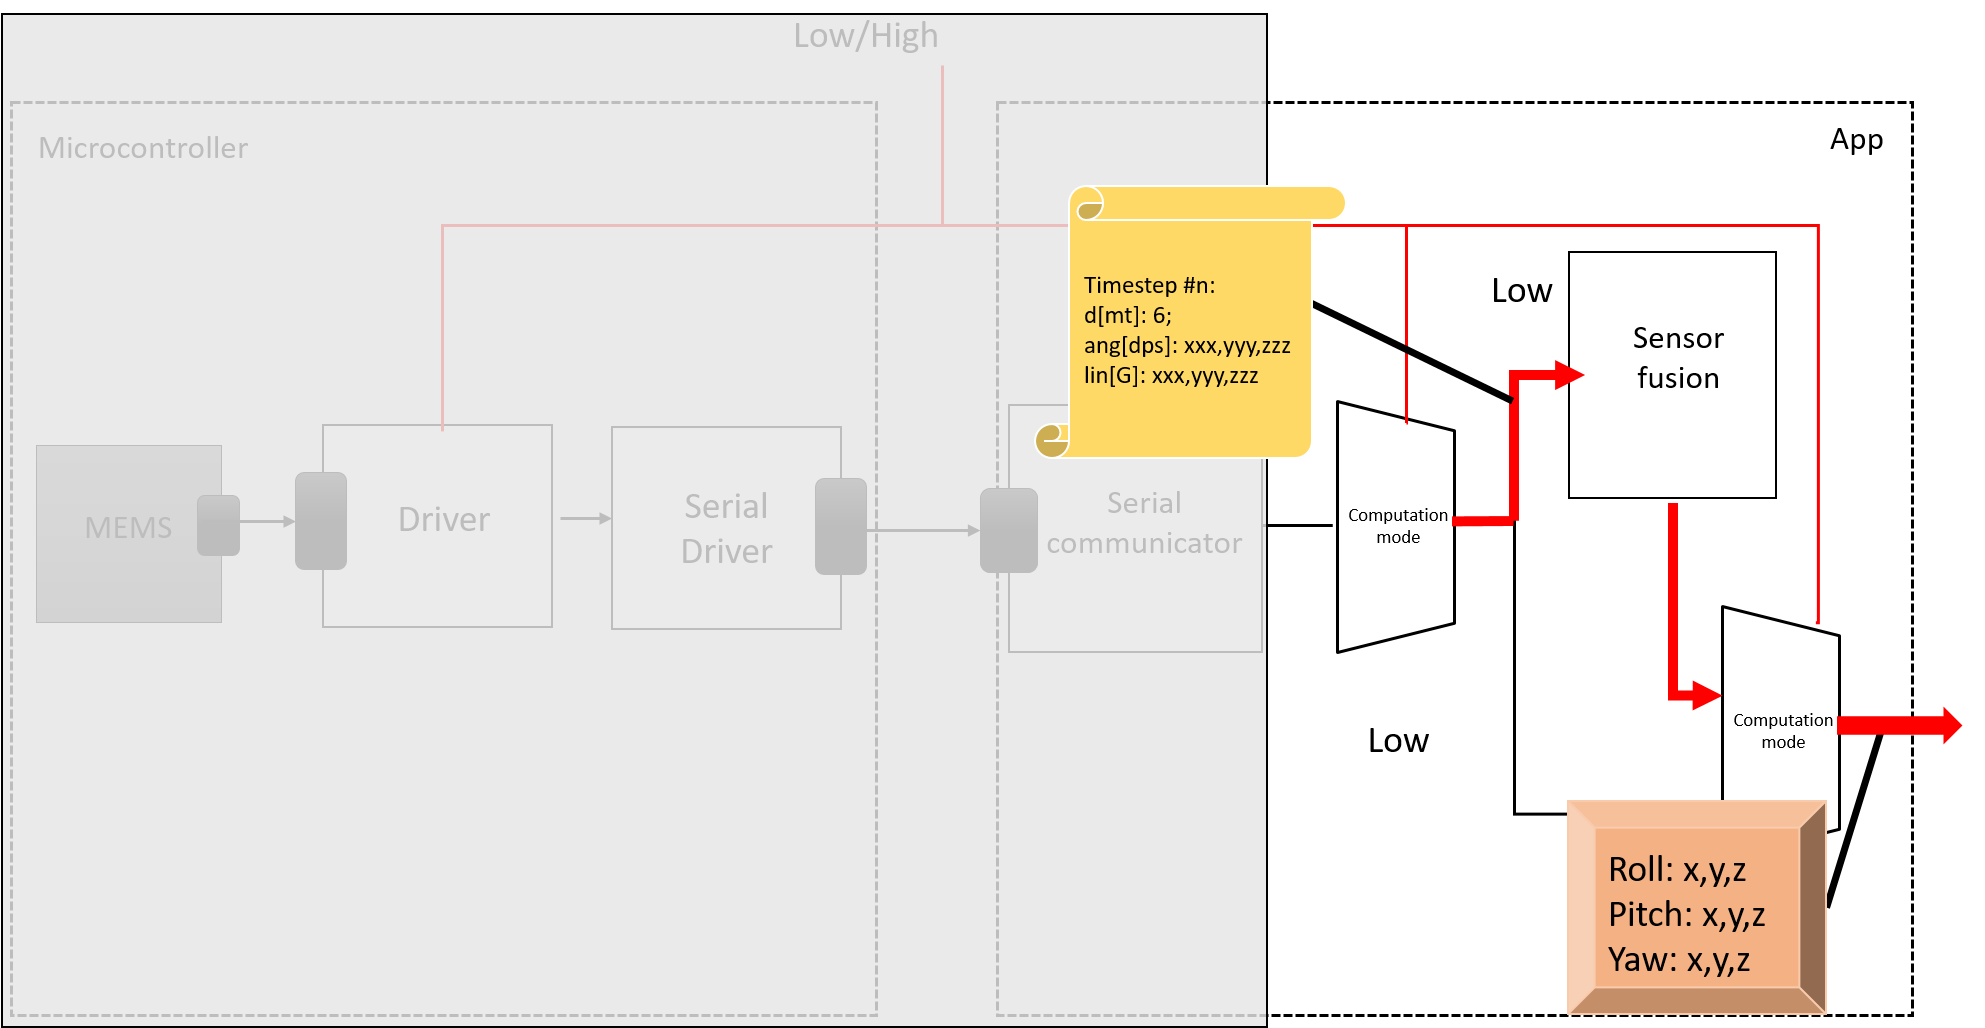
\includegraphics[scale=0.25 ]{DescrizioneDelSistema/flusso3.png}
 	\caption{Rappresentazione del flusso di dati tra i moduli dei sottosistemi, step 3}
 	\label{fig:flusso3}
 \end{figure}
\newpage
A questo punto il modulo \textit{Sensor Fusion} elabora i dati grezzi (vedi cap.\ref{sensor_fusion}) fornendo in uscita gli angoli di Eulero (Cap.\ref{assetto}) relativi all'operatore:
\begin{itemize}
	\item \textbf{Roll}
	\item \textbf{Pitch}
	\item \textbf{Yaw} 
\end{itemize}
Questi dati verranno usati come input dal sottosistema S2 (si veda \ref{fig:sistema_liv1}) che provvederà, insieme all'informazione relativa alla distanza dal nodo precedente, a determinare l'angolo del nuovo nodo e quindi a risolvere il problema di georeferenziazione emerso nel livello di astrazione precedente (si veda \ref{livello_sottosistemi}).
